\documentclass[aps,prl,twocolumn,superscriptaddress,nofootinbib]{revtex4-2}
\usepackage{amsmath,amssymb,amsfonts}
\usepackage{graphicx}
\usepackage{hyperref}
\usepackage{braket}

%% Canonical theorem / module / Aristotle counts. Regenerated by
%% scripts/update_counts.py. Use \totaltheorems{}, \aristotleproved{},
%% \leanmodules{}, \axiomcount{} instead of inline literals.
% Auto-generated by update_counts.py — 2026-04-24T19:44:03.140400
% Do not edit manually. Run: uv run python scripts/update_counts.py
\newcommand{\totaltheorems}{3993}
\newcommand{\substantivetheorems}{3882}
\newcommand{\placeholdertheorems}{111}
\newcommand{\axiomcount}{1}
\newcommand{\sorrycount}{0}
\newcommand{\sorrypercent}{0.0}
\newcommand{\leanmodules}{167}
\newcommand{\leandefinitions}{3297}
\newcommand{\pythonmodules}{68}
\newcommand{\testfiles}{59}
\newcommand{\totaltests}{2836}
\newcommand{\figurecount}{111}
\newcommand{\notebookcount}{54}
\newcommand{\papercount}{19}
\newcommand{\aristotleproved}{322}
\newcommand{\aristotleruns}{44}
% --- Paper 18 / Phase 5t per-section counts (FermiHubbardDimer.lean) ---
\newcommand{\fhdTotal}{143}
\newcommand{\fhdWaveTwo}{13}
\newcommand{\fhdWaveThree}{6}
\newcommand{\fhdWaveFour}{22}
\newcommand{\fhdWaveFive}{22}
\newcommand{\fhdWaveSixABC}{38}
\newcommand{\fhdWaveSixExtra}{15}
\newcommand{\fhdWaveSeven}{19}
\newcommand{\fhdWaveEight}{8}

\newcommand{\mathlibcommit}{\mathlibrev}

\begin{document}

\title{Three Generations of Standard-Model Fermions from Modular Invariance:\\
A Machine-Checked Derivation}

\author{John G. Roehm}
\affiliation{Independent Researcher}
\email{jgroehm@gmail.com}

\date{\today}

\begin{abstract}
Two global conditions force the Standard Model's generation count to
satisfy $N_f \equiv 0 \pmod 3$, with $N_f = 3$ the smallest nonzero
solution: the chiral central charge $c_- = 8 N_f$, set by the $16$
left-handed Weyl components per generation, and $24 \mid c_-$, from
modular invariance of the reduced partition function. The chain is
kernel-checked in Lean~4, with the $8$ derived from the component count
rather than assumed. Without right-handed neutrinos the two conditions
collapse onto one and each excludes three generations alone, so either
they exist or a compensating sector carries the deficit.
\end{abstract}

\maketitle

%% ══════════════════════════════════════════════════════════════════
\section{Introduction}

The Standard Model contains three generations of fermions, and its
perturbative gauge anomalies cancel within each generation
independently~\cite{GrossJackiw1972}. Nothing at that level
distinguishes three from one, two, or four.

Wang~\cite{Wang2024} proposed that a global condition does. Under
dimensional reduction the Standard Model's Weyl content fixes the
chiral central charge of a two-dimensional theory at $c_- = 8 N_f$,
while modular invariance of that theory's torus partition function
requires $24 \mid c_-$. The two conditions meet in the factorization
$24 = 8 \times 3$: the physical factor cancels and the residue
$N_f \equiv 0 \pmod 3$ survives, with $N_f = 3$ the smallest nonzero
solution. The proposal recasts an empirical count as the minimal output
of a consistency requirement, and it is falsifiable by any internally
consistent extension of the Standard Model that violates it.

This Letter reports that chain checked by the Lean~4 kernel against
Mathlib, and two things the check makes precise. The coefficient $8$ is
derived rather than supplied: the theorem that produces it takes the
sum over the Standard Model's multiplets as its argument, not the
numeral $16$. And the counterfactual in which right-handed neutrinos
are absent turns out to be overdetermined. Modular invariance and the
global anomaly are usually presented as independent conditions to be
imposed together; at fifteen Weyl components per generation they
collapse onto the same divisibility, and each excludes three
generations without help from the other. Throughout, $c_-$ denotes the
total chiral central charge over all $N_f$ generations, and $\sigma$
the signature of the intersection form of a closed $4$-manifold.

%% ══════════════════════════════════════════════════════════════════
\section{The fermion content fixes $c_- = 8 N_f$}
\label{sec:central_charge}

We work in the convention in which each generation carries a
right-handed neutrino. Its left-handed Weyl content is then the quark
doublet $Q_L$ at $(\mathbf{3}, \mathbf{2})$, the antiquark singlets
$\bar{u}_R$ and $\bar{d}_R$ at $(\bar{\mathbf{3}}, \mathbf{1})$, the
lepton doublet $L$ at $(\mathbf{1}, \mathbf{2})$, and the
charged-lepton and neutrino singlets $\bar{e}_R$ and $\bar{\nu}_R$ at
$(\mathbf{1}, \mathbf{1})$, giving $6+3+3+2+1+1 = 16$ components.

These descend to two dimensions by a domain-wall mechanism of
Jackiw--Rebbi type: a mass profile that reverses sign across a wall
localizes on it a massless fermion carrying half the bulk degrees of
freedom, and iterating the construction from five dimensions down to
two carries each $4$d Weyl component to exactly one $1+1$d
Majorana--Weyl fermion~\cite[Sec.~II\,A]{Wang2024}. The counting is
one-to-one at every step, which is what lets the anomaly be read off
downstairs. Each Majorana--Weyl fermion carries chiral central charge
$1/2$~\cite[Eqs.~(6)--(11)]{Wang2024}, so one generation contributes
$16 \times \tfrac{1}{2} = 8$ and $N_f$ generations contribute
$c_- = 8 N_f$.

The coefficient $8$ is not an input. The multiplet content is declared
in \texttt{SMFermionData.lean} as an inductive type together with a
component-count function, and the central charge is the function
$n \mapsto n/2$ on that count. The theorem
\texttt{fermion\_count\_gives\_central\_charge}, in
\texttt{WangBridge.lean}, states
\begin{equation*}
\texttt{weyl\_central\_charge}
\Big( \textstyle\sum_{f} \texttt{components}\, f \Big) = 8 ,
\end{equation*}
the sum running over those multiplets. Its argument is that sum and not
the numeral $16$, so the $8$ is the value the content takes under the
reduction rather than a coefficient supplied by hand. The formalization
fixes the per-generation value, and the passage to $c_- = 8 N_f$ is the
additivity of the central charge over $N_f$ identical copies; that last
step is arithmetic we do not machine-check.

Dropping the right-handed neutrino leaves $15$ components per
generation, and the same function returns $15/2$:
\texttt{chiral\_charge\_without\_nu\_R} states
$\texttt{weyl\_central\_charge}\,15 = 15/2$, so in that case
$c_- = 15 N_f / 2$, a half-integer whenever $N_f$ is odd.

%% ══════════════════════════════════════════════════════════════════
\section{Modular invariance forces $3 \mid N_f$}
\label{sec:framing}

The second ingredient is a divisibility on $c_-$, and together with
$c_- = 8 N_f$ it leaves three as the smallest admissible generation
count.

The Dedekind eta function is
\begin{equation}
\eta(\tau) = q^{1/24} \prod_{n=1}^{\infty}(1 - q^n),
\qquad q = e^{2\pi i \tau},
\end{equation}
and under the modular $T$-transformation $\tau \to \tau + 1$ it
acquires a phase, $\eta(\tau+1) = e^{2\pi i/24}\,\eta(\tau)$. The two
factors behave differently. Since $q(\tau+1) = q(\tau)$, the infinite
product is unchanged, and the entire phase comes from the prefactor
$q^{1/24}$. That exponential identity is what is machine-checked:
\texttt{qParam\_shift}, in \texttt{ModularInvarianceConstraint.lean},
states $\exp(2\pi i (z+1)/h) = \exp(2\pi i/h)\exp(2\pi i z/h)$ for
$h \neq 0$ and reduces it to Mathlib's \texttt{Complex.exp\_add}. At
$h = 24$ it supplies the eta prefactor's phase; at $h = 1$ it is the
invariance of $q$.

The $24$ admits two readings that agree. Analytically it is the
exponent of the $q$-expansion prefactor displayed above. Physically it
is the Casimir energy of the two-dimensional conformal vacuum on the
torus, $E_0 = -c/24$, whose $24$ traces to the zeta-regularized value
$\zeta(-1) = -1/12$ in the Virasoro central
term~\cite[Eq.~(16) and n.~9]{Wang2024}.

The torus partition function carries the central charge in the same
place,
$Z(\tau) = \mathrm{Tr}\, q^{L_0 - c/24}\,\bar{q}^{\bar{L}_0 -
\bar{c}/24}$~\cite[Eq.~(15)]{Wang2024}, so under $T$ it returns
$Z(\tau+1) = e^{2\pi i c_-/24}\,Z(\tau)$ with $c_- = c - \bar{c}$.
Modular invariance is the requirement that this phase equal $1$, and
that requirement is exactly a divisibility:
\texttt{framing\_anomaly\_constraint}, in the same module, states
$e^{2\pi i c/24} = 1 \iff 24 \mid c$ for integer $c$, so invariance and
divisibility are equivalent rather than one merely sufficient for the
other.

Substituting $c_- = 8 N_f$ turns the condition into arithmetic,
\begin{equation}
24 \mid 8 N_f \quad \Longleftrightarrow \quad 3 \mid N_f .
\label{eq:gen_constraint}
\end{equation}
\texttt{modular\_generation\_constraint} discharges this step, taking
$24 \mid 8 N_f$ as a hypothesis and returning $3 \mid N_f$. The modular
condition is physical input to that theorem rather than a consequence
of it; what the kernel certifies is the arithmetic passage.

The step is sharp at the bottom of the range, one and two generations
being excluded by the same computation that admits three
(\texttt{constraint\_sharpness}, and Fig.~\ref{fig:phase}).
\texttt{twenty\_four\_decomposition} records the factorization
$24 = 8 \times 3$ with $\gcd(8,3) = 1$, separating the two inputs: $24$
is mathematical, fixed by zeta regularization and carried by the eta
prefactor, while $8$ is physical, fixed by the multiplet content of
Sec.~\ref{sec:central_charge}. Because $3$ is coprime to $8$, the
residue that survives cancellation constrains the generation count
alone and adds nothing the fermion count already implies.

Three is therefore the minimal nonzero solution
(\texttt{generation\_minimal\_nontrivial}, in
\texttt{GenerationConstraint.lean}). The observed
$N_f = 3$ is not fitted here; it is the minimum of the set that
Eq.~\eqref{eq:gen_constraint} leaves.

\begin{figure}[t]
\centering
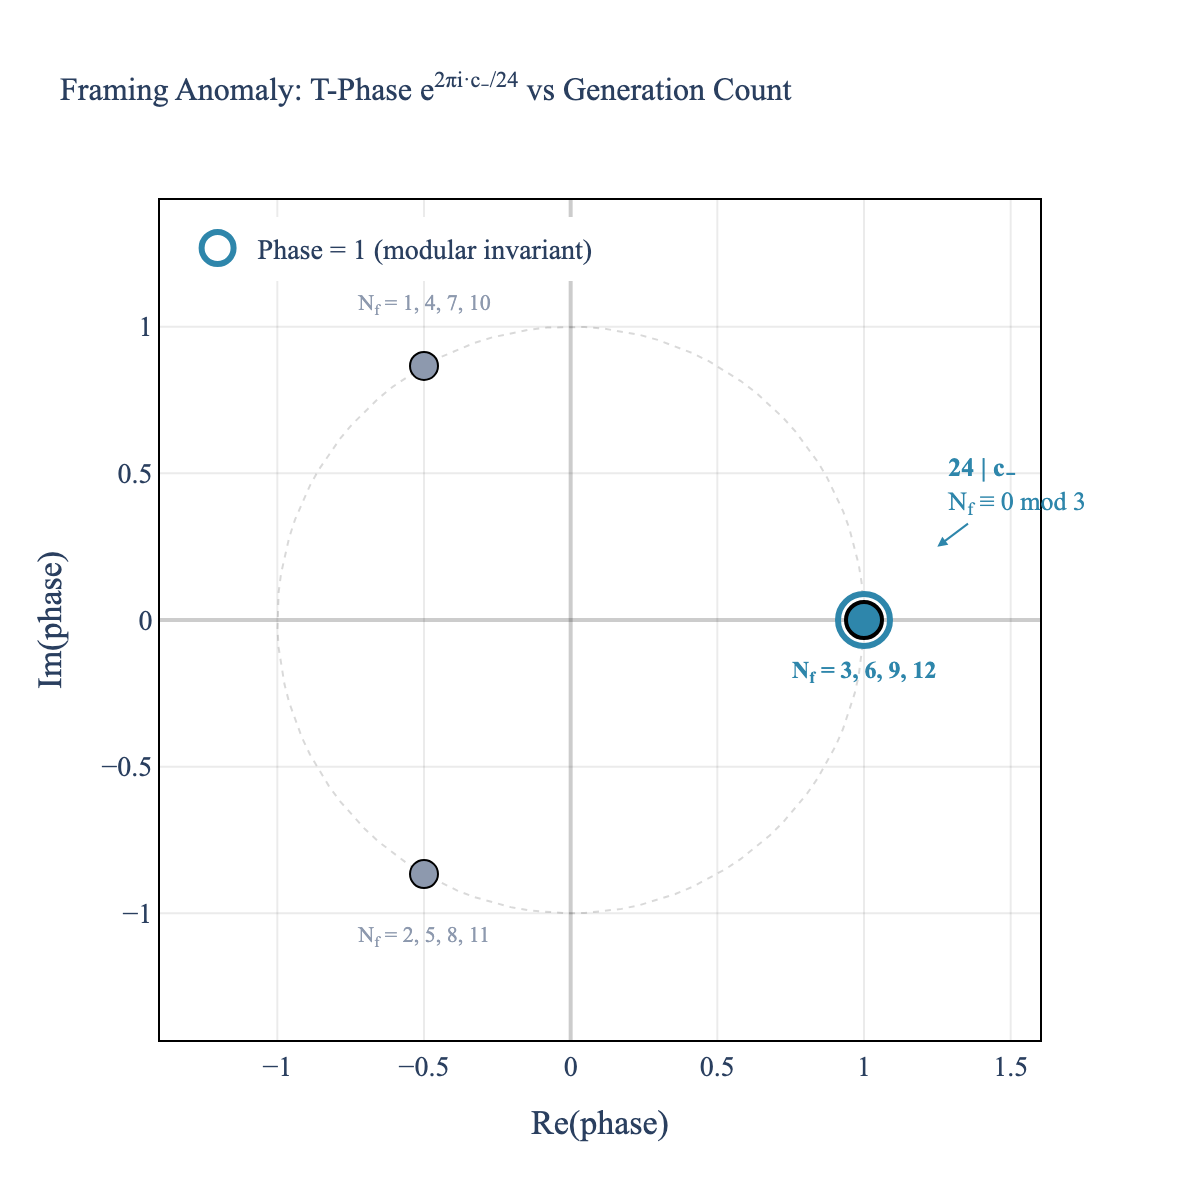
\includegraphics[width=\columnwidth]{figures/fig75_modular_invariance_phase.png}
\caption{The $T$-transformation phase $e^{2\pi i c_-/24}$ at
$c_- = 8 N_f$, which reduces to $e^{2\pi i N_f/3}$ and so takes only
the three cube roots of unity. The phase equals $1$ (blue ring, modular
invariant) exactly for $N_f \in \{3,6,9,12\}$; the grey markers carry
the excluded counts $N_f \in \{1,4,7,10\}$ and
$N_f \in \{2,5,8,11\}$.}
\label{fig:phase}
\end{figure}

%% ══════════════════════════════════════════════════════════════════
\section{Right-handed neutrinos, or a sector carrying the deficit}
\label{sec:nur}

Modular invariance is not the only global condition the Standard Model
must satisfy, and the second one is sensitive to exactly the field the
first is not. With a right-handed neutrino present every Standard-Model
fermion carries charge $1 \bmod 4$ under the $\mathbb{Z}_4$ combination
$X = -2Y + 5(B-L)$, so the Standard Model admits a
$\mathrm{Spin}^{\mathbb{Z}_4}$ structure and its global anomaly is
classified by $\Omega_5^{\mathrm{Spin}^{\mathbb{Z}_4}} \cong
\mathbb{Z}_{16}$~\cite[Sec.~4.3]{GarciaEtxebarria2019}, an interacting
classification rather than a free-fermion one. Sixteen unit charges per
generation then sum to zero
in $\mathbb{Z}_{16}$ for every $N_f$, which
\texttt{z16\_anomaly\_always\_cancels\_with\_nu\_R} records. That
constraint is therefore empty in the with-$\nu_R$ convention, modular
invariance is the whole of what remains, and the minimal generation
count is $3$.

Remove the right-handed neutrino and fifteen charges per generation
must sum to zero instead. Since $15$ is a unit modulo $16$, this is a
genuine restriction: \texttt{z16\_anomaly\_without\_nu\_R} states
$15 N_f \equiv 0 \pmod{16}$ if and only if $16 \mid N_f$.

Modular invariance does not soften that conclusion, and it does not
combine with it either. The residue $3 \mid N_f$ of
Sec.~\ref{sec:framing} is a consequence of $c_- = 8 N_f$, which is the
sixteen-component spectrum; at fifteen components the central charge is
$c_- = 15 N_f/2$ instead. For odd $N_f$ that is not an integer at all,
so at three families $c_- = 45/2$ and the theory carries a
gravitational anomaly outright;
\texttt{central\_charge\_fractional\_without\_nu\_R} records the
one-generation value by deriving a contradiction from the assumption
that $15/2$ is a natural number. For even $N_f = 2m$ the requirement
becomes $24 \mid 15 m$, and since $5$ is a unit modulo $8$ this is
again $16 \mid N_f$. The two conditions therefore coincide rather than
compound, each excluding $N_f = 3$ on its own, and the smallest
generation count consistent with either is sixteen.

An observed $N_f = 3$ is thus incompatible with a spectrum of exactly
fifteen Weyl components per generation \emph{and nothing else}. The
alternative is not excluded, and both cited sources name it. A
topological sector can absorb the deficit without adding local degrees
of freedom: Ref.~\cite{GarciaEtxebarria2019} notes that Dai--Freed
constraints are altered by Green--Schwarz terms or, more generally, by
coupling to a suitable topological field theory, and
Wang~\cite{Wang2024} identifies the concrete candidate for the case at
hand, a Pfaffian-like non-Abelian quantum Hall sector supplying the
missing $c_- = 3/2$ in the reduced bulk, which is the per-generation
shortfall $8 - 15/2 = 1/2$ taken three times. The constraint therefore reads
as a disjunction: either right-handed neutrinos are present, or a
compensating sector carries the deficit. Both horns are sharp, and
distinguishing them is a question about physics beyond the Standard
Model rather than about the derivation. One scope condition attaches to
the $\mathbb{Z}_{16}$ leg throughout: a Majorana mass for $\nu_R$
breaks $B-L$, and electroweak symmetry breaking breaks $X$ as well, so
the classification constrains the ultraviolet spectrum rather than the
low-energy one~\cite[Sec.~4.3]{GarciaEtxebarria2019}.

One remark on why the divisor above is sixteen and not eight. The
$4$-manifold shadow of $\mathbb{Z}_{16}$ is Rokhlin's theorem: the
signature of a closed smooth spin $4$-manifold is divisible by $16$,
not merely by $8$~\cite{Rokhlin1952}. An even unimodular intersection
form alone delivers $8 \mid \sigma$, and \texttt{eight\_dvd\_latticeSig}
derives that much from unimodularity by van der Blij's argument, with
the Hasse--Minkowski and theta-modularity inputs discharged. The extra
factor of two is assumed rather than derived, as it must be:
$16 \mid \sigma$ is false for general even unimodular forms, $E_8$
having $\sigma = 8$, and a closed topological $4$-manifold carrying
that form consequently admits no smooth structure. Granting evenness of
the $\hat{A}$-genus, \texttt{SmoothSpinManifold4.rokhlin} proves
$16 \mid \sigma$ on Lean's standard axioms alone; the K3 surface
saturates the bound at $\sigma = -16$. The route from
$\mathbb{Z}_{16}$ down to that signature statement runs through ko
cohomology of a point~\cite{Adams1974}, convergence of the Adams
spectral sequence~\cite{BeaudryCampbell} and the
Anderson--Brown--Peterson splitting~\cite{ABP1967}, which enter here as
established results rather than as formalized ones.

None of this reaches Secs.~\ref{sec:central_charge} and
\ref{sec:framing}. The headline $3 \mid N_f$ rests on the fermion
content and the modular condition alone, and carries neither the
topological input nor the bridge results just disclosed.

%% ══════════════════════════════════════════════════════════════════
\section{Discussion}

The divisibility $24 \mid c_-$ admits a deeper reading, in which
it is a corollary of the classification of meromorphic conformal field
theories at $c = 24$~\cite{Schellekens1993}, geometrically completed
for the strongly rational, weight-one-nontrivial subset by
M\"oller and Scheithauer~\cite{MollerScheithauer2024}, rather than a
stand-alone modular-consistency requirement. A companion paper on
anomaly constraints on Standard-Model particle content carries that
derivation~\cite{Roehm2026D2}.

The Standard Model's generation count appears here as the smallest
solution of a divisibility that modular invariance imposes on a
quantity the fermion content fixes. Wang states the conclusion in that
register, as a count the conditions favor, and observes that the
constraint may bear on the low-energy spectrum
alone~\cite[Sec.~IV]{Wang2024}. Read either way it is falsifiable: an
internally consistent extension of the Standard Model whose fermion
content violates $N_f \equiv 0 \pmod 3$ refutes it.

\begin{acknowledgments}
The author thanks the Mathlib community, whose modular-forms and
linear-algebra libraries this development builds on.
\end{acknowledgments}

\section*{Artifact availability, methods and tools}
Every theorem cited above is in the public repository accompanying this
work, and reproduces under \texttt{lake build} with Lean~4
v\leantoolchain\ against Mathlib commit \texttt{\mathlibcommit{}}. The
matrix identities in the Steenrod-algebra development are discharged by
\texttt{native\_decide}, which trusts Lean's compiled evaluator rather
than its kernel; everything the argument above rests on is checked by
the kernel on its standard axioms.

The formal verification layer was developed with substantial machine
assistance: Lean~4 proof drafting and iteration used LLM-based agents
(Anthropic Claude-family models). Every proof is ultimately certified
by the kernel independently of any such tool. Manuscript prose was
AI-assisted and human-reviewed.

\begin{thebibliography}{99}
\bibitem{Wang2024}
J.~Wang, ``Family Puzzle, Framing Topology, $c_-=24$ and
$3(E_8)_1$ Conformal Field Theories: $48/16 = 45/15 = 24/8 = 3$,''
arXiv:2312.14928 (2023).

\bibitem{GrossJackiw1972}
D.~Gross and R.~Jackiw,
Phys.\ Rev.\ D \textbf{6}, 477 (1972).

\bibitem{GarciaEtxebarria2019}
I.~Garc\'ia-Etxebarria and M.~Montero,
JHEP \textbf{08}, 003 (2019) [arXiv:1808.00009].

\bibitem{Rokhlin1952}
V.~Rokhlin, Dokl.\ Akad.\ Nauk SSSR \textbf{84}, 221 (1952).

\bibitem{Adams1974}
J.~F.~Adams,
\emph{Stable Homotopy and Generalised Homology}
(University of Chicago Press, 1974).

\bibitem{ABP1967}
D.~W.~Anderson, E.~H.~Brown~Jr., and F.~P.~Peterson,
Ann.\ Math.\ \textbf{86}, 271 (1967).

\bibitem{BeaudryCampbell}
A.~Beaudry and J.~A.~Campbell,
Contemp.\ Math.\ \textbf{718}, 89 (2018)
[arXiv:1801.07530].

\bibitem{Schellekens1993}
A.~N.~Schellekens,
``Meromorphic $c=24$ conformal field theories,''
Comm.\ Math.\ Phys.\ \textbf{153}, 159 (1993),
arXiv:hep-th/9205072.

\bibitem{MollerScheithauer2024}
S.~M\"oller and N.~R.~Scheithauer,
``A geometric classification of the holomorphic vertex operator
algebras of central charge $24$,''
Algebra \& Number Theory \textbf{18}, 1891 (2024),
arXiv:2112.12291.

\bibitem{Roehm2026D2}
J.~Roehm, ``Anomaly constraints on Standard Model particle content,''
in preparation (2026).

\end{thebibliography}

\end{document}
